\documentclass{standalone}

\usepackage[siunitx,americanvoltages, europeanresistors,americancurrents]{circuitikz}
\usepackage{color}
\usepackage{graphicx}%Für Grafiken
\usepackage{rotating} % lässt Grafiken rotieren
\usepackage{mathtools}% mathematische Werkzeuge
\usepackage{amsmath}% Mathetools
\usepackage{amsfonts}% Mathetools
\usepackage{physics}
\usepackage{amssymb}% Symbole wie Natürliche Zahlen
\usepackage{geometry}
\usepackage{caption} % Unter-/Überschriften für Bilder, Grafiken und Tabellen
\usepackage{tikz}
\usepackage{amsthm}

% tikz libraries
\usetikzlibrary{arrows}
\usetikzlibrary{3d}
\usetikzlibrary{angles, quotes, shapes, decorations.markings, calc, arrows.meta}

% mathmatical commands
\newcommand{\AAA}{\mathbf{A}}
\newcommand{\R}{\mathbb{R}}
\newcommand{\N}{\mathbb{N}}
\newcommand{\p}{\mathcal{P}}
\newcommand{\I}{\infty}
\newcommand{\ve}{\varepsilon}
\newcommand{\vp}{\varphi}

\begin{document}
	
	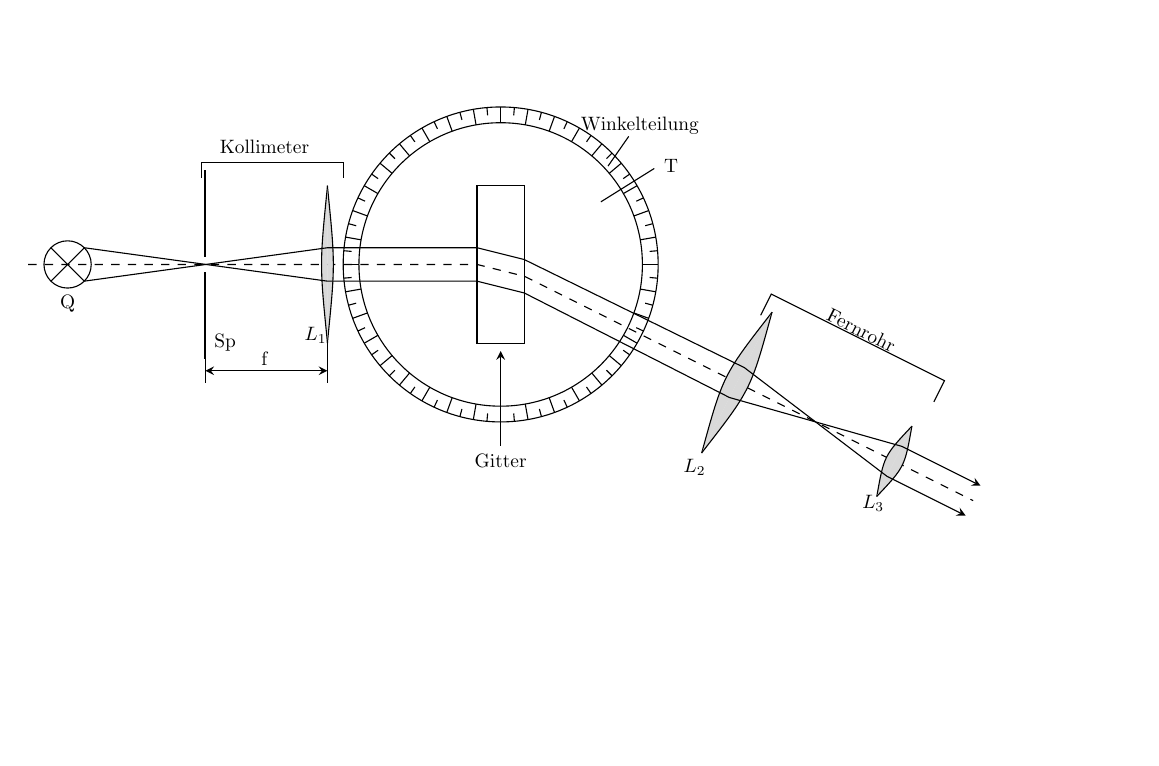
\begin{tikzpicture}[>=stealth]
		\draw[white] (-6,-6) rectangle (8,3);
		\draw[dashed] (-6,0) -- (-.3,0) -- (.3,-.15) -- (6,-3);
		
		% Winkelteilung
		\draw (0,0) circle (1.8);
		\draw (0,0) circle (2);
		\foreach \x in {0,10,...,350}
		\draw[thin] ({cos(\x)*1.8},{sin(\x)*1.8}) -- ({cos(\x)*2},{sin(\x)*2});
		\foreach \x in {5,15,...,355}
		\draw[thin] ({cos(\x)*1.9},{sin(\x)*1.9}) -- ({cos(\x)*2},{sin(\x)*2});
		
		% Gitter
		\draw (-.3,-1) rectangle (.3,1);
		
		% Linsen
		
		\filldraw[draw=black, fill=gray!30!white] (-2.201,1) .. controls (-2.1,0) .. (-2.201,-1);
		\filldraw[draw=black, fill=gray!30!white] (-2.199,1) .. controls (-2.3,0) .. (-2.199,-1);
		\filldraw[draw=black, fill=gray!30!white] ({cos(90-26.565)*1+3.0001},{sin(90-26.565)*1-1.500}) .. controls ({cos(180-26.565)*0.1+2.91324},{sin(180-26.565)*0.1-1.45216}) .. ({cos(270-26.565)*1+3.0001},{sin(270-26.565)*1-1.500});
		
		\filldraw[draw=black, fill=gray!30!white] ({cos(90-26.565)*1+2.999},{sin(90-26.565)*1-1.500}) .. controls ({cos(0-26.565)*0.1+3.08676},{sin(-26.565)*0.1-1.54804}) .. ({cos(270-26.565)*1+2.999},{sin(270-26.565)*1-1.500});
		
		\filldraw[draw=black, fill=gray!30!white] ({cos(90-26.565)*0.5+5.0001},{sin(90-26.565)*0.5-2.500}) .. controls ({cos(180-26.565)*0.05+4.91324},{sin(180-26.565)*0.05-2.45216}) .. ({cos(270-26.565)*0.5+5.0001},{sin(270-26.565)*0.5-2.500});
		
		\filldraw[draw=black, fill=gray!30!white] ({cos(90-26.565)*0.5+4.999},{sin(90-26.565)*0.5-2.500}) .. controls ({cos(0-26.565)*0.05+5.08676},{sin(-26.565)*0.05-2.54804}) .. ({cos(270-26.565)*0.5+4.999},{sin(270-26.565)*0.5-2.500});
		
		
		% Q
		\draw (-5.5,0) circle (0.3);
		\draw[->] 
		({-5.5+cos(225)*0.3},{sin(225)*.3}) -- 
		({-5.5+cos(45)*0.3},{sin(45)*.3}) -- 
		(-2.2,-0.2121320) -- 
		(-.3,-0.2121320) -- 
		(.3,-.362132) -- 
		({cos(270-26.565)*0.212132+3},{sin(270-26.565)*0.212132-1.5}) -- 
		({cos(90-26.565)*0.212132+5},{sin(90-26.565)*0.212132-2.500}) -- 
		({cos(90-26.565)*0.212132+6},{sin(90-26.565)*0.212132-3});
		
		\draw[->] ({-5.5+cos(135)*0.3},{sin(135)*.3}) --
		({-5.5+cos(315)*0.3},{sin(315)*.3}) -- 
		(-2.2,0.2121320) -- 
		(-0.3,0.2121320) -- 
		(.3,.062132) -- 
		({cos(90-26.565)*0.212132+3},{sin(90-26.565)*0.212132-1.5}) -- 
		({cos(270-26.565)*0.212132+5},{sin(270-26.565)*0.212132-2.500}) -- 
		({cos(270-26.565)*0.212132+6},{sin(270-26.565)*0.212132-3});
		
		% Sp
		\draw[thick] (-3.75,0.1) -- (-3.75,1.2);
		\draw[thick] (-3.75,-0.1) -- (-3.75,-1.2);
		
		% Kollimeter
		\draw (-3.8,1.1) -- (-3.8,1.3) -- (-2,1.3) -- (-2,1.1);
		\draw[very thin] (-3.75,-1.2) -- (-3.75,-1.5);
		\draw[very thin] (-2.2,-1) -- (-2.2,-1.5);
		\draw[<->] (-3.75,-1.35) -- (-2.2,-1.35);
		
		
		% Fernrohr
		\draw ({2.9+cos(90-26.565)*0.9},{-1.45+sin(90-26.565)*0.9}) -- ({2.9+cos(90-26.565)*1.2},{-1.45+sin(90-26.565)*1.2}) -- ({5.1+cos(90-26.565)*1.2},{-2.55+sin(90-26.565)*1.2}) -- ({5.1+cos(90-26.565)*.9},{-2.55+sin(90-26.565)*.9});
		
		% Beschriftungen
		\node[scale=0.7,rotate=-26.565] at ({4.+cos(90-26.565)*1.3},{-2.+sin(90-26.565)*1.3}) {Fernrohr\index{Fernrohr}};
		\node[scale=0.7] at (-3,1.5) {Kollimeter\index{Kollimeter}};
		\node[scale=.7] at (0,-2.5) {Gitter\index{Gitter}\label{Bes: Gitter}};
		\draw[->] (0,-2.3) -- (0,-1.1);
		\node[scale=0.7] at ({cos(45)*2.5},{sin(45)*2.5}) {Winkelteilung\index{Winkelteilung}};
		\draw ({cos(45)*2.3},{sin(45)*2.3}) -- ({cos(42.5)*1.85},{sin(42.5)*1.85});
		\node[scale=.7] at (-5.5,-0.5) {Q};
		\node[scale=.7] at (-3.5,-1) {Sp};
		\node[scale=.7] at (-2.35,-.9) {$ L_1 $};
		\node[scale=.7] at (-3,-1.2) {f};
		\node[scale=.7] at ({cos(30)*2.5},{sin(30)*2.5}) {T};
		\draw ({cos(32)*1.5},{sin(32)*1.5}) -- ({cos(32)*2.3},{sin(32)*2.3});
		\node[scale=.7] at ({cos(270-26.565)*1.2+3},{sin(270-26.565)*1.2-1.5}) {$ L_2 $};
		\node[scale=.7] at ({cos(270-26.565)*0.6+5},{sin(270-26.565)*0.6-2.5}) {$ L_3 $};
	\end{tikzpicture}
	
\end{document}
